%%%%%%%%%%%%%%%%%%%%%%%%%%%%%%%%%%%%%%%%%
% 
% LaTeX Template
% Version 3.1 (25/3/14)
%
%%%%%%%%%%%%%%%%%%%%%%%%%%%%%%%%%%%%%%%%%

%----------------------------------------------------------------------------------------
%	PACKAGES AND DOCUMENT CONFIGURATIONS
%----------------------------------------------------------------------------------------

\documentclass[12pt, a4 paper]{article}

\usepackage{tikz}
%\usepackage[top=2cm, bottom=2cm, outer=0cm, inner=0cm]{geometry}
\usepackage{graphicx} % Required for the inclusion of images
\usepackage{multicol} % Required for multicolumns
\usepackage{setspace} % Required for line spacing
\setlength\parindent{0pt} % Removes all indentation from paragraphs
\setlength{\columnseprule}{0.4pt} % Adds vertical line between multicolumns
\usepackage{multirow} % Required for multirows
\usepackage{booktabs} % For prettier tables
\usepackage{xcolor}
%\usepackage{tabularx}
%\renewcommand{\rmdefault}{ptm}

%\usepackage{helvet}

\usepackage{times} % Uncomment to use the Times New Roman font

%----------------------------------------------------------------------------------------
%	DOCUMENT INFORMATION
%----------------------------------------------------------------------------------------

\begin{document}

\tikz[remember picture,overlay] \node[inner sep=0pt] at (current page.center){
\includegraphics[width=\paperwidth,height=\paperheight]{image.png}};

\clearpage

%\font\myfont=cmr12 at 35pt
%\title{\myfont  Event Name} % Write Event name here
%\author{}
%\date{\vspace{-10ex}}

%\maketitle % Insert the title, author and date
\setstretch{1.5}

%\tikz[remember picture,overlay] \node[opacity=0.8,inner sep=0pt] at (current page.center){
\includegraphics[width=\paperwidth,height=\paperheight]{Border48-A4--Arvin61r58.png}};
%\tikz[remember picture,overlay] \node[opacity=0.5,inner sep=0pt] at (current page.center){\includegraphics[width=\paperwidth,height=\paperheight]{color-2174049__340.png}};

\begin{center}
\Huge \bfseries \ttfamily SPLASH
\end{center}

\begin{center}
\large Celebrating Technical Holi
\end{center}

\begin{center}
\begin{multicols}{2}
\begin{tabular}{l r}
Date: & March 19,2019\\ % Date the event was held
Time: & 3:00 PM to 5:00 PM \\ % Time of event 
\end{tabular}
\columnbreak
\begin{tabular}{l r}
Venue: & G-12 \\ % Venue of event
Total Attendance: & 25 \\ % Number of participants
\end{tabular}
\end{multicols}


\begin{LARGE}
F.R.I.E.N.D Zone 		POP n DROP
\end{LARGE}

\begin{Large}
\begin{multicols}{2}
An event named SPLASH was organized on March 19,2019 from 3:00 PM to 5:00 PM in room G-12 (MBA Block) of the college. The event consisted of two rounds :
\columnbreak
%\includegraphics[width=\linewidth]{placeholder.jpg}
  %\caption{A boat.}
  %\label{fig:boat1}
\end{multicols}

\begin{multicols}{2}

%\includegraphics[width=\linewidth]{placeholder.jpg}

\columnbreak
In first round, there was an online quiz relating Friends web-series. There were 20 questions in total including audio related questions and mcq’s. 
\end{multicols}

\newpage 

%\tikz[remember picture,overlay] \node[opacity=0.8,inner sep=0pt] at (current page.center){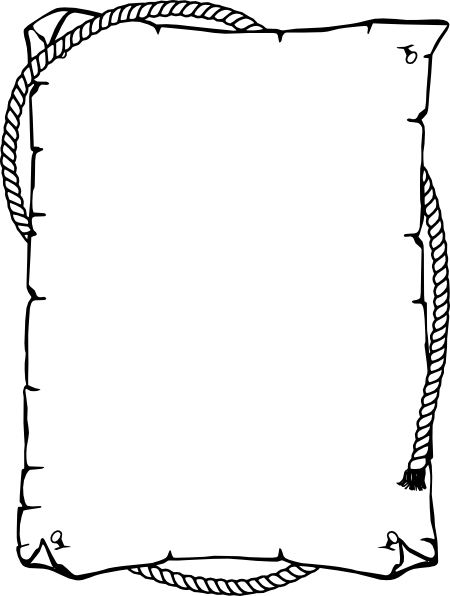
\includegraphics[width=\paperwidth,height=\paperheight]{5TRrp44jc.png}};
%\tikz[remember picture,overlay] \node[opacity=0.8,inner sep=0pt] at (current page.center){\includegraphics[width=\paperwidth,height=\paperheight]{md_5b0912b7c0870.png}};

\begin{multicols}{2}
About 12 students qualified for the second round. In second round, the qualified students had to burst the balloons in order to find the clues which leaded them to their questions. 
\columnbreak
%\includegraphics[width=\linewidth]{placeholder.jpg}
  
\end{multicols}

\begin{multicols}{2}
%\includegraphics[width=\linewidth]{placeholder.jpg}

\columnbreak
  The questions were present in the form of puzzles related to some famous company logos. 
\end{multicols} 

\begin{multicols}{2}
The students had to solve the puzzle and recognize the logo names. The complete event was interesting.

\columnbreak
%\includegraphics[width=\linewidth]{placeholder.jpg}
  
\end{multicols} 
  
\end{Large} 
\end{center}

\newpage 

%\tikz[remember picture,overlay] \node[opacity=0.8, inner sep=0pt] at (current page.center){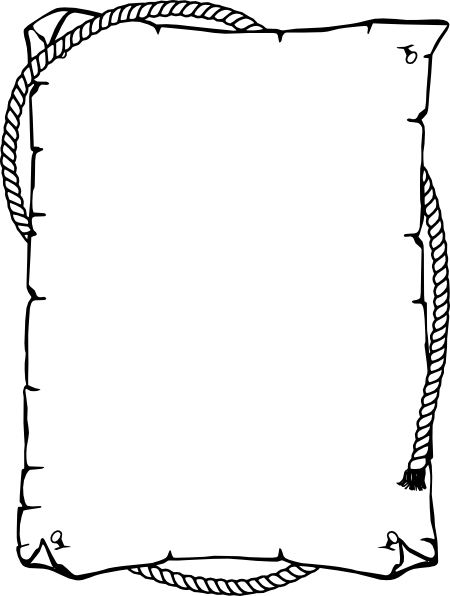
\includegraphics[width=\paperwidth,height=\paperheight]{5TRrp44jc.png}};
%\tikz[remember picture,overlay] \node[opacity=0.8,inner sep=0pt] at (current page.center){\includegraphics[width=\paperwidth,height=\paperheight]{md_5b0912b7c0870.png}};

\begin{center}
\Huge Pictures Section
\end{center}

\newpage 

\tikz[remember picture,overlay] \node[opacity=0.8,inner sep=0pt] at (current page.center){
\includegraphics[width=\paperwidth,height=\paperheight]{image1.png}};

\newpage

\tikz[remember picture,overlay] \node[opacity=0.8,inner sep=0pt] at (current page.center){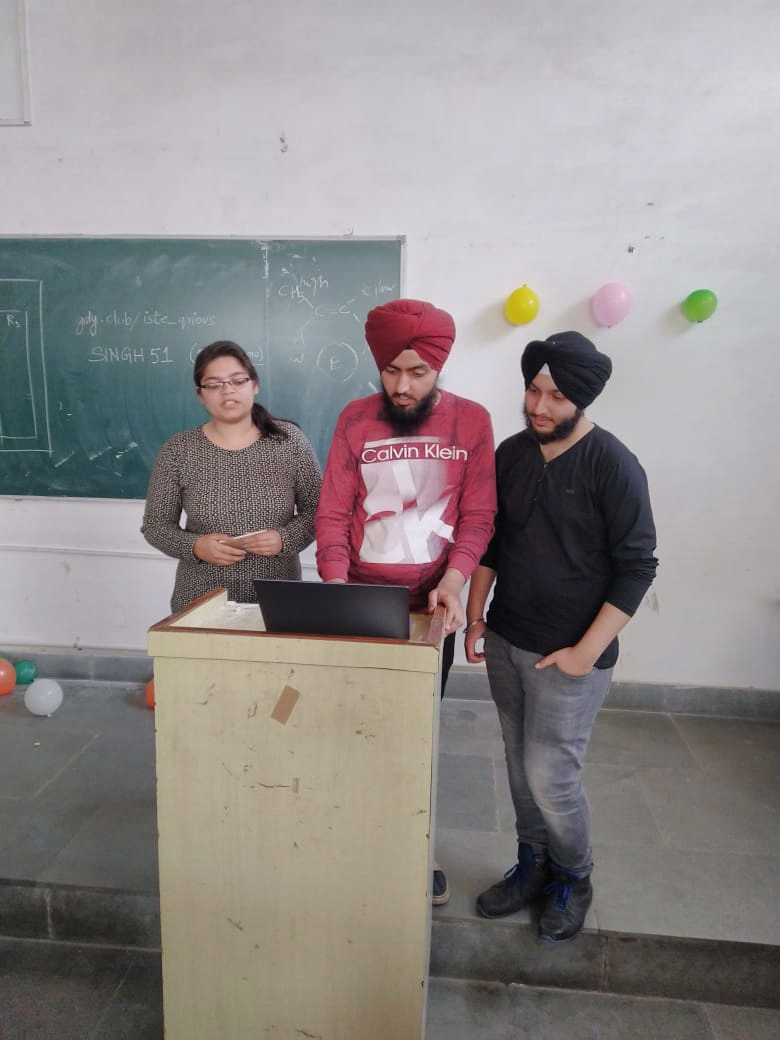
\includegraphics[width=\paperwidth,height=\paperheight]{image2.png}};


\newpage

\tikz[remember picture,overlay] \node[opacity=0.8,inner sep=0pt] at (current page.center){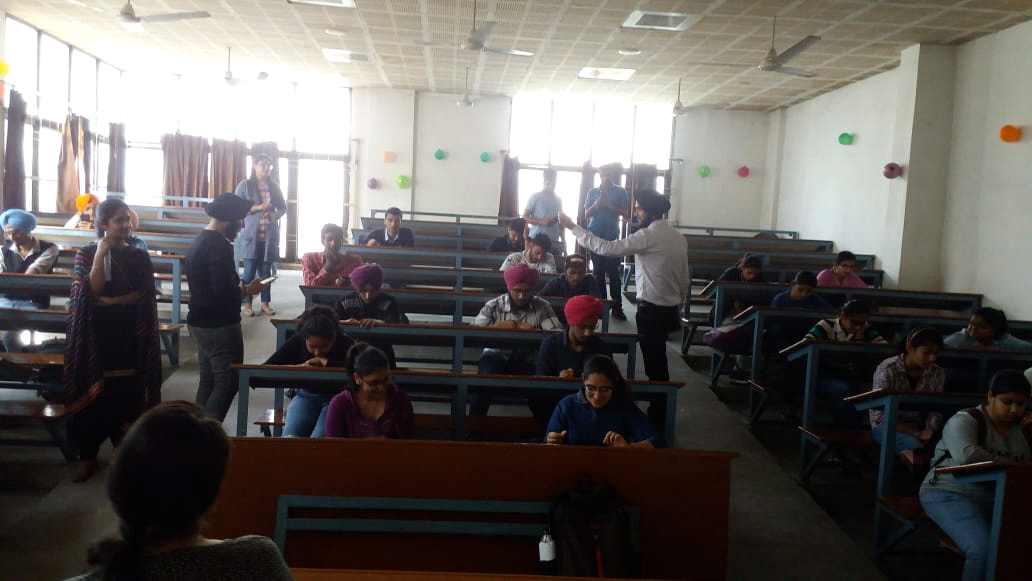
\includegraphics[width=\paperwidth,height=\paperheight]{image3.png}};

\newpage

\begin{center}
\huge Organisers list
\end{center}

\begin{table}[h!]
  \begin{center}
    \begin{tabular}{|c|c|c|c|c|c|} 
    \toprule % <-- Toprule here
      \textbf{S.No.} & \textbf{Name} & \textbf{Branch/Year} & \textbf{Roll No.} \\
      \midrule % <-- Midrule here
      1 & Harmanjot kaur & D2 ECE & 1706726 \\
      2 & Alok Kumar  & D2 ME & 1706945  \\
      3 & Sudhanshu Dubey & D2 CSE & 1706523  \\
      4 & Kiratpreet Singh & D2 ECE & 1706741 \\
      5 & Jagmeet Singh  & D2 ECE & 1706728 \\
      6 & Amrit Kaur  & D2 ECE  & 1706705     \\
      7 & Kamya Arora & D2 CSE  & 1706453   \\
      8 & Paridhi     & D2 CSE  & 1706485  \\

      \bottomrule % <-- Bottomrule here
    \end{tabular}
  \end{center}
\end{table}


\begin{center}
\huge Management list
\end{center}

\begin{table}[h!]
  \begin{center}
    \begin{tabular}{|c|c|c|c|c|c|} 
    \toprule % <-- Toprule here
      \textbf{S.No.} & \textbf{Name} & \textbf{Branch/Year} & \textbf{Roll No.} \\
      \midrule % <-- Midrule here
      1 & Avi Sehgal           & D3 CSE & 1606655 \\
      2 & Darshpreet Singh     & D3 CSE & 1606668 \\
      3 & Shubham Baranwal     & D3 IT  & 1607156 \\
      4 & Shivam Srivastava    & D3 IT  & 1607155 \\
      6 & Ishpreet Kaur Gulati & D2 CSE & 1706443 \\
      7 & Dilnish Kaur         & D2 ECE & 1706721 \\
      8 & Parneet Kaur         & D2 CSE & 1706486 \\

      \bottomrule % <-- Bottomrule here
    \end{tabular}
  \end{center}
\end{table}

\newpage

\tikz[remember picture,overlay] \node[opacity=0.8,inner sep=0pt] at (current page.center){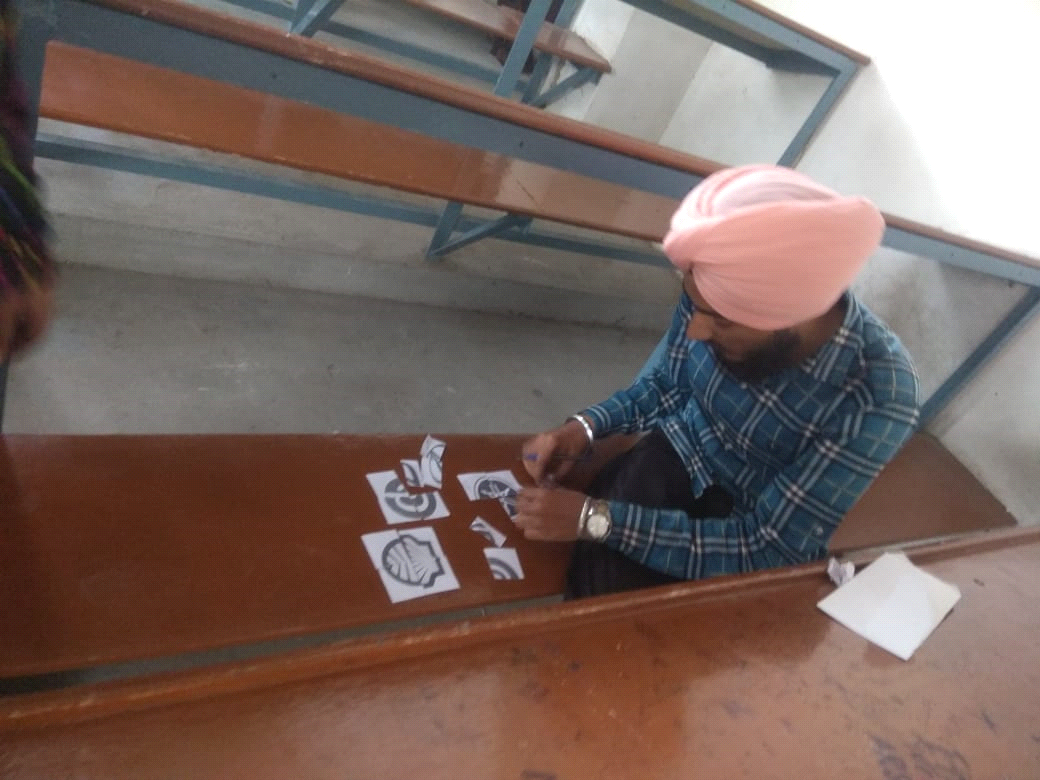
\includegraphics[width=\paperwidth,height=\paperheight]{image4.png}};

\newpage

\tikz[remember picture,overlay] \node[opacity=0.8,inner sep=0pt] at (current page.center){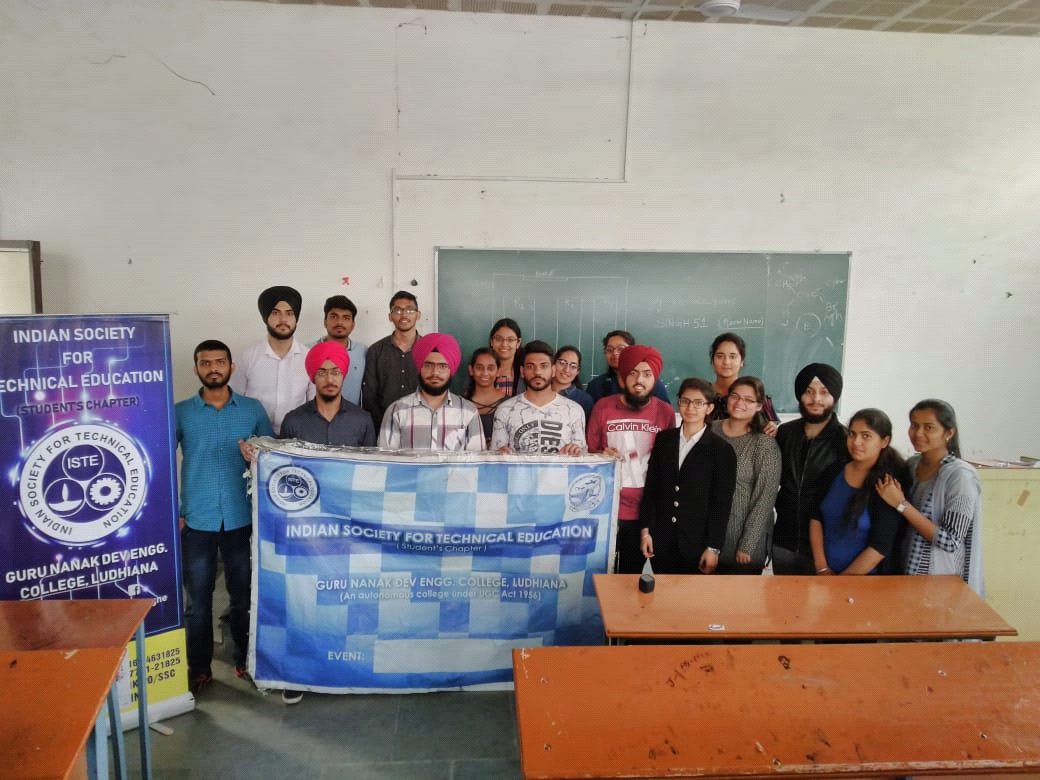
\includegraphics[width=\paperwidth,height=\paperheight]{image5.png}};

\newpage

\begin{center}
\huge Winners List
\end{center}

\begin{table}[h!]
  \begin{center}
    \begin{tabular}{|c|c|c|c|c|c|} 
    \toprule % <-- Toprule here
      \textbf{S.No.} & \textbf{Name} & \textbf{Branch/Year} & \textbf{Roll No.} &\textbf{Position} \\
      \midrule % <-- Midrule here
      1 & Lakshay Chopra  & D2 CSE   & 1706462 & 1st \\
      2 & Shahbaz Singh   & D1 CSE   & 1815073 & 2nd \\
      3 & Gurashish Singh & D3 CIVIL & 1606445 & 3rd \\

      \bottomrule % <-- Bottomrule here
    \end{tabular}
  \end{center}
\end{table}

\newpage

\begin{center}
\huge Participant list
\end{center}

\begin{table}[h!]
  \begin{center}
    \begin{tabular}{|c|c|c|c|c|c|} 
    \toprule % <-- Toprule here
      \textbf{S.No.} & \textbf{Name} & \textbf{Branch/Year} \\
      \midrule % <-- Midrule here
      1 & Lakshay Chopra    & D2 CSE \\          
      2 & Shahbaz Singh     & D1 CSE \\         
      3 & Gurashish Singh   & D3 CE  \\   
      4 & Satinder Singh    & D1 CSE \\
      5 & Rajat Kumar       & D1 CSE \\
      6 & Adarsh            & D1 CSE \\
      7 & Mayank Thakur     & D1 CSE \\
      8 & Shruti            & D1 ECE \\
      9 & Srishti           & D1 ECE \\
     10 & Mokshi            & D1 ECE \\
     11 & Tanisha           & D1 ECE \\
     12 & Avleen            & D1 ECE \\
     13 & Harnoor Singh     & D1 ECE \\
     14 & Sukhjinder Singh  & D1 ECE \\
     15 & Simaranjeet Singh & D1 ECE \\
     16 & Aashish Kumar     & D1 ECE \\
     17 & Simaranjeet kaur  & D1 ECE \\
     18 & Rohit Sohata      & D1 ECE \\
     19 & Rita              & D1 ECE \\
     20 & Simaranjeet kaur  & D1 ECE \\
     21 & Manveen Kaur      & D4 CSE \\
     22 & Nitya Garg        & D4 CSE \\
     23 & Vasudha           & D1 CSE \\
     24 & Shivani           & D1 CSE \\
     25 & Aditya Raj Sharma & D1 CSE \\

      \bottomrule % <-- Bottomrule here
    \end{tabular}
  \end{center}
\end{table}


\end{document}